\documentclass[11pt, a4paper]{article}
\usepackage{sectsty}
\usepackage{graphicx}
\usepackage{amsmath}
\usepackage{amssymb}
\usepackage{setspace}
\usepackage{tasks}
\usepackage{graphicx}
\usepackage{float}
\usepackage{comment}
\usepackage{listings}
\usepackage[utf8]{inputenc}
\usepackage{amsfonts}
\usepackage{gensymb}
\usepackage{multicol}
\usepackage{tabularx}
\usepackage{tikz}
\newcommand{\myvec}[1]{\ensuremath{\begin{pmatrix}#1\end{pmatrix}}}
\let\vec\mathbf
\newcommand{\abs}[1]{\left| #1 \right|}
\newcommand{\mydet}[1]{\ensuremath{\begin{vmatrix}#1\end{vmatrix}}}
\providecommand{\brak}[1]{\ensuremath{\left(#1\right)}}
\providecommand{\lbrak}[1]{\ensuremath{\left(#1\right.}}
\providecommand{\rbrak}[1]{\ensuremath{\left.#1\right)}}
\providecommand{\cbrak}[1]{\ensuremath{\left\{#1\right\}}}
\providecommand{\sbrak}[1]{\ensuremath{{}\left[#1\right]}}
\providecommand{\norm}[1]{\left\lVert#1\right\rVert}
\providecommand{\abs}[1]{\left\vert#1\right\vert}
\usepackage[left=1in, right=0.5in, top=1in, bottom=1in]{geometry}
\title{ Math computing}
\author{ Yaswanth }
\date{\today}

\begin{document}
\vspace{-\baselineskip}
\maketitle

\section*{NCERT 9.7.1.5}

\textbf{This question is from class 9 ncert chapter 7.triangles}
\begin{enumerate}
    \item Line $l$ is the bisector of an angle $\angle A$ and $B$ is any point on $l$. $BP$ and $BQ$ are perpendiculars from $B$ to the arms of $\angle A$. Show that:
%
\begin{enumerate}
    \item $\triangle  APB \cong \triangle AQB$  
    \item $BP$ = $BQ$ or $B$ is equidistant from the arms of $\angle A$.
 \end{enumerate}
\end{enumerate}
\begin{figure}[H]
    \centering
    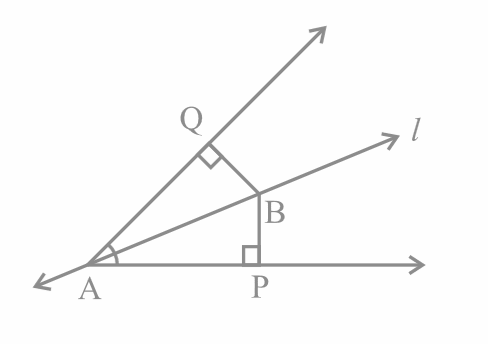
\includegraphics[width=1\columnwidth]{fig_mc.png}
    \caption{$\triangle AQB \hspace{12pt} and \hspace{12pt} \triangle APB$}
    \label{fig:math_comp1}
\end{figure}
\pagebreak

%
\begin{enumerate}
\item \textbf{Finding foot of perpendiculars $P,Q$ using Eigen Approach:} 


Assuming that the point $A$ be the intersection point of two tangents of a circle with centre $B$ and radius $r$. Let consider $P,Q$ be the points of contact of two tangents to the circle.

\begin{table}[H]
\begin{center}
 \begin{tabular}{|c|c|p{6cm}|}
	 \hline  \label{tab:table2}
        \textbf{Symbol} & \textbf{Value} & \textbf{Description} \\
        \hline
	 $\vec{A}$ & $\myvec{0 \\ 0}$ & coordinates of vertex $A$ \\
        \hline
	 $\vec{B}$ & $\myvec{3 \\ 3}$ & centre of circle $B$ \\
        \hline
        $r$ & $2$ & radius of circle \\
        \hline
    \end{tabular}
\end{center}
\caption{parameters for eigen approach}
%\label{tab:table2}
\end{table}

\begin{enumerate}

\item let ,consider $h = A$ and $u=-B$
\begin{align}
	\vec{h} &=\vec{A} \label{eq:h} \\
	\vec{u} &=\vec{-B} \\
	\vec{h} &=\myvec{a \\ b} \\
\vec{u} &= \myvec{c \\ d}  \\
	\vec{V} &= \myvec{1 & 0 \\ 0 & 1} \\
	\vec{f} &= \norm{u}^2-r^2   \label{eq:f}
\end{align}

\item finding the circle equation: 
\begin{align}
	\vec{gh} &= \vec{h^T}\vec{V}\vec{h} + 2\vec{u^T}\vec{h} + f    \label{eq:gh}\\
	\vec{gh} &= \myvec{a &b}\myvec{1 & 0 \\ 0 & 1}\myvec{a \\ b} + 2\myvec{c& d}\myvec{a \\b } + f   \label{eq:gh2} \\
\end{align}

\item from Table \ref{tab:table2} and \eqref{eq:h}, 
\begin{align}
\vec{h} &=\myvec{0 \\ 0} \\
\vec{u} &= \myvec{-3 \\ -3} \\
r &= 2 
\end{align}
\item on substituting these in \eqref{eq:f} and  \eqref{eq:gh2} we get,
\begin{align}
\vec{f} &=14.000000 \\
\vec{gh} &= \myvec{0 &0 }\myvec{1 & 0 \\ 0 & 1}\myvec{0 \\ 0} + 2\myvec{-3& -3}\myvec{0 \\0 } + 14.0 \\
\vec{gh} &= 14.000000  
\end{align}

\item Finding the sigma matrix : 
\begin{align}
	\vec{\Sigma} &= \brak{\vec{V}\vec{h}+\vec{u}}\brak{\vec{V}\vec{h}+\vec{u}}^T -\vec{gh}\vec{V}  \label{eq:sigmat}\\
	\vec{\Sigma} &= \brak{\myvec{1 &0 \\0 & 1}\myvec{a \\ b}+\myvec{c \\ d}} \brak{\myvec{1 &0 \\0 & 1}\myvec{a \\b}+\myvec{c \\ d}}^T - \vec{gh}\myvec{1 &0 \\ 0& 1}   \label{eq:sigmat2} \\
\intertext{on substituting we get  }   \nonumber \\ 
	\vec{\Sigma} &= \brak{\myvec{1 &0 \\ 0 &1}\myvec{0 \\ 0 }+\myvec{-3 \\  -3}} \brak{\myvec{1 &0 \\ 0&1}\myvec{0 \\ 0}+\myvec{-3 \\ -3}}^T - 14.0 \myvec{1 &0 \\ 0& 1 } \\
	&= \myvec{-5.000000  & 9.000000 \\ 9.000000 & -5.000000 } \label{eq:sigmat3}
\end{align}

\item  Finding eigen values and eigen vectors for \eqref{eq:sigmat3} ,we get 
	\begin{align}
		\vec{\lambda} &=\myvec{4\\-14} \\
		\vec{\lambda_1} &=4 \\
		\vec{\lambda_2} &=-14  \\
		\vec{P} &=\myvec{ -0.707107& -0.707107\\ -0.707107 & 0.707107} 
	\end{align}

\item Finding  The direction vectors of the tangents from a point h to the circle
\begin{align}
	\vec{m} &=\vec{P}\myvec{\sqrt{\abs{\lambda_2}}\\ \pm \sqrt{\abs{\lambda_1}}} \\
		&=\myvec{ -0.707107& -0.707107\\ -0.707107 & 0.707107}\myvec{\sqrt{\abs{-14}}\\ \pm \sqrt{\abs{4}}} \\
\intertext{on solving  we get  }   \nonumber \\ 
	\vec{m_1} &=\myvec{-4.059965 \\ -1.231538 } \\
	\vec{m_2} &=\myvec{-1.231538 \\ -4.059965 } 
\end{align}

\item Finding  the contact points 
	\begin{align}
		\vec{x}=\vec{h}+\vec{\mu}\vec{m} \\
\intertext{Here  }   \nonumber \\
		\vec{\mu} &=-\frac{\vec{m^T}\brak{\vec{V}\vec{h}+u}}{\vec{m^T}\vec{V}\vec{m}}  \\
		\vec{\mu_1} &=-\frac{\vec{m_1^T}\brak{\vec{V}\vec{h}+u}}{\vec{m_1^T}\vec{V}\vec{m_1}} \\
		\vec{\mu_2} &=-\frac{\vec{m_2^T}\brak{\vec{V}\vec{h}+u}}{\vec{m_2^T}\vec{V}\vec{m_2}} \\
		\vec{\mu_1} &=-\frac{ \myvec{ -4.059965 & -1.231538}\brak{\myvec{1 &0 \\0 &1}\myvec{0 \\0}+\myvec{-3 \\-3}}}{\myvec{-4.059965 & -1.231538} \myvec{1 &0 \\ 0 & 1}\myvec{-4.059965 \\ -1.231538}} \\
		\vec{\mu_2} &=-\frac{ \myvec{ -1.231538 & -4.059965}\brak{\myvec{1 &0 \\0 &1}\myvec{0 \\0}+\myvec{-3 \\-3}}}{\myvec{-1.231538 & -4.059965} \myvec{1 &0 \\ 0 & 1}\myvec{-1.231538 \\ -4.059965}} \\
\intertext{on solving we get, }   \nonumber \\
		\vec{\mu_1} &=-0.881917 \\
		\vec{\mu_2} &=-0.881917
	\end{align}

\item now for contact points $P$ and $Q$
	\begin{align}
		\vec{P} &=\vec{h}+\vec{\mu_1}\vec{m_1} \\
		\vec{Q} &=\vec{h}+\vec{\mu_2}\vec{m_2} \\
		\vec{P} &=\myvec{0 \\0}+\myvec{-0.881917}\myvec{-4.059965 \\ -1.231538} \\
		\vec{Q} &=\myvec{0 \\0}+\myvec{-0.881917}\myvec{-1.231538 \\ -4.059965} \\
		\vec{P} &=\myvec{ 3.580552\\ 1.086114} \\
		\vec{Q} &=\myvec{ 1.086114\\ 3.580552} 
	\end{align}

\item As the lines $BP$ and $BQ$ are radius of circle ,So the lengths of  $BP$ and $BQ$ are  equal 
\end{enumerate}

\begin{figure}[H]
    \centering
    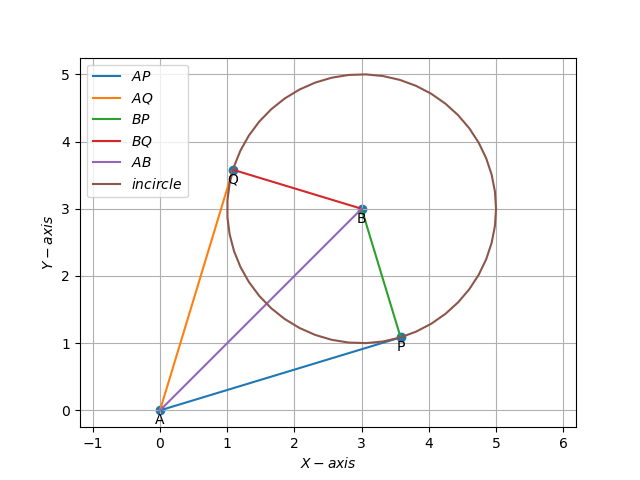
\includegraphics[width=1\columnwidth]{eigen.png}
    \caption{Contact points $P$ and $Q$}
    \label{fig:eigen}
\end{figure}

\end{enumerate}





\end{document}
